
\حصہء{سوالات}
\موٹا{ترسیم شدہ تفاعل کا تجزیہ}\\
سوال \حوالہ{سوال_استعمال_نشاندہی_الف} تا سوال \حوالہ{سوال_استعمال_نشاندہی_چ} میں دیے ترسیم کی نقطہ تصریف، مقامی کم سے کم اور مقامی زیادہ سے زیادہ نقطہ کی نشاندہی کریں۔ ان وقفوں کہ نشاندہی کریں جن پر ترسیم اوپر مقعر اور جن پر نیچے مقعر ہے۔ 

\ابتدا{سوال}\شناخت{سوال_استعمال_نشاندہی_الف}
\عددی{y=\tfrac{x^3}{3}-\tfrac{x^2}{2}-2x+\tfrac{1}{3}}، شکل \حوالہ{شکل_سوال_استعمال_نشاندہی_الف}
\انتہا{سوال}
%=======================
\ابتدا{سوال}\شناخت{سوال_استعمال_نشاندہی_ب}
\عددی{y=\tfrac{x^4}{4}-2x^2+4}، شکل \حوالہ{شکل_سوال_استعمال_نشاندہی_ب}
\انتہا{سوال}
%==========================
\ابتدا{سوال}\شناخت{سوال_استعمال_نشاندہی_پ}
\عددی{y=\tfrac{3}{4}(x^2-1)^{2/3}}، شکل \حوالہ{شکل_سوال_استعمال_نشاندہی_پ}
\انتہا{سوال}
%==========================
\ابتدا{سوال}\شناخت{سوال_استعمال_نشاندہی_ت}
\عددی{y=\tfrac{9}{14}x^{1/3}(x^2-7)}، شکل \حوالہ{شکل_سوال_استعمال_نشاندہی_ت}
\انتہا{سوال}
%==========================
\ابتدا{سوال}\شناخت{سوال_استعمال_نشاندہی_ٹ}
\عددی{y=x+\sin 2x,\, -\tfrac{2\pi}{3}\le x\le \tfrac{2\pi}{3}}، شکل \حوالہ{شکل_سوال_استعمال_نشاندہی_ٹ}
\انتہا{سوال}
%==========================
\ابتدا{سوال}\شناخت{سوال_استعمال_نشاندہی_ث}
\عددی{y=\tan x-4x,\,-\tfrac{\pi}{2}<x<\tfrac{\pi}{2}}، شکل \حوالہ{شکل_سوال_استعمال_نشاندہی_ث}
\انتہا{سوال}
%==========================
\ابتدا{سوال}\شناخت{سوال_استعمال_نشاندہی_ج}
\عددی{y=\sin \abs{x},\, -2\pi\le x\le 2\pi}، شکل \حوالہ{شکل_سوال_استعمال_نشاندہی_ج}
\انتہا{سوال}
%==========================
\ابتدا{سوال}\شناخت{سوال_استعمال_نشاندہی_چ}
\عددی{y=2\cos x-\sqrt{2}x,\,-\pi\le x\le \tfrac{3\pi}{2}}، شکل \حوالہ{شکل_سوال_استعمال_نشاندہی_چ}
\انتہا{سوال}
%==========================


\begin{figure}
\centering
\begin{minipage}{0.22\textwidth}
\centering
\begin{tikzpicture}[font=\small]
\begin{axis}[width=4cm,font=\tiny,axis lines=middle,xlabel={$x$},ylabel={$y$},ylabel style={at={(current axis.above origin)},anchor=south},xtick={\empty},ytick={\empty}]
\addplot[domain=-3:4.5]{x^3/3-x^2/2-2*x+1/3}node[pos=0.7,above left,fill=white]{$y=\tfrac{x^3}{3}-\tfrac{x^2}{2}-2x+\tfrac{1}{3}$};
\end{axis}
\end{tikzpicture}
\caption{}
\label{شکل_سوال_استعمال_نشاندہی_الف}
\end{minipage}\hfill
\begin{minipage}{0.22\textwidth}
\centering
\begin{tikzpicture}[font=\small]
\begin{axis}[width=4cm,font=\tiny,axis lines=middle,xlabel={$x$},ylabel={$y$},ylabel style={at={(current axis.above origin)},anchor=south},xtick={\empty},ytick={\empty}]
\addplot[domain=-3.5:3.5,smooth]{x^4/4-2*x^2+4}node[pos=0.7,above left,fill=white]{$y=\tfrac{x^4}{4}-2x^2+4$};
\end{axis}
\end{tikzpicture}
\caption{}
\label{شکل_سوال_استعمال_نشاندہی_ب}
\end{minipage}\hfill
\begin{minipage}{0.22\textwidth}
\centering
\begin{tikzpicture}[font=\small]
\begin{axis}[width=4cm,font=\tiny,axis lines=middle,xlabel={$x$},ylabel={$y$},ylabel style={at={(current axis.above origin)},anchor=south},xtick={\empty},ytick={\empty}]
\addplot[domain=-2:2,smooth]{3/4*((x^2-1)^2)^(1/3)}node[pos=0.85,above left,fill=white]{$y=\tfrac{3}{4}(x^2-1)^{2/3}$};
\end{axis}
\end{tikzpicture}
\caption{}
\label{شکل_سوال_استعمال_نشاندہی_پ}
\end{minipage}\hfill
\begin{minipage}{0.22\textwidth}
\centering
\begin{tikzpicture}[font=\small]
\begin{axis}[clip=false,width=4cm,font=\tiny,axis lines=middle,xlabel={$x$},ylabel={$y$},ylabel style={at={(current axis.above origin)},anchor=south},xtick={\empty},ytick={\empty}]
\addplot[domain=0:0.1,smooth]{9/14*x^(1/3)*(x^2-7)};
\addplot[domain=0:0.1,smooth]({-x},{-9/14*x^(1/3)*(x^2-7)});
\addplot[domain=0.1:4,smooth]{9/14*x^(1/3)*(x^2-7)};
\addplot[domain=0.1:4,smooth]({-x},{-9/14*x^(1/3)*(x^2-7)})node[pos=0.9,below right,fill=white]{$y=\tfrac{9}{14}x^{1/3}(x^2-7)$};
\end{axis}
\end{tikzpicture}
\caption{}
\label{شکل_سوال_استعمال_نشاندہی_ت}
\end{minipage}
\end{figure}
%
\begin{figure}
\centering
\begin{minipage}{0.22\textwidth}
\centering
\begin{tikzpicture}[font=\small]
\begin{axis}[clip=false,width=4cm,font=\tiny,axis lines=middle,xlabel={$x$},ylabel={$y$},ylabel style={at={(current axis.above origin)},anchor=south},xtick={-2.094,2.094},xticklabels={$-\tfrac{2\pi}{3}$,$\tfrac{2\pi}{3}$},ytick={\empty},xmin=-2.5,xmax=3]
\addplot[domain=-2.092:2.094,smooth]{x+sin(deg(2*x))}node[pos=0.5,above left,fill=white]{$y=x+\sin 2x$};
\end{axis}
\end{tikzpicture}
\caption{}
\label{شکل_سوال_استعمال_نشاندہی_ٹ}
\end{minipage}\hfill
\begin{minipage}{0.22\textwidth}
\centering
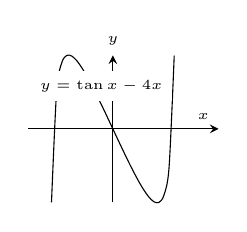
\begin{tikzpicture}[font=\small]
\begin{axis}[clip=false,width=4cm,font=\tiny,axis lines=middle,xlabel={$x$},ylabel={$y$},ylabel style={at={(current axis.above origin)},anchor=south},xtick={\empty},ytick={\empty},xmin=-2,xmax=2.5]
\addplot[domain=-1.45:1.45,smooth]{tan(deg(x))-4*x}node[pos=0.9,above left,fill=white]{$y=\tan x-4x$};
\end{axis}
\end{tikzpicture}
\caption{}
\label{شکل_سوال_استعمال_نشاندہی_ث}
\end{minipage}\hfill
\begin{minipage}{0.22\textwidth}
\centering
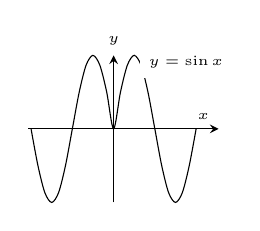
\begin{tikzpicture}[font=\small]
\begin{axis}[clip=false,width=4cm,font=\tiny,axis lines=middle,xlabel={$x$},ylabel={$y$},ylabel style={at={(current axis.above origin)},anchor=south},xtick={\empty},ytick={\empty},xmin=-6.5,xmax=8]
\addplot[domain=-6.284:6.284,smooth]{sin(deg(abs(x)))}node[pos=0.65,right,fill=white]{$y=\sin\abs{x}$};
\end{axis}
\end{tikzpicture}
\caption{}
\label{شکل_سوال_استعمال_نشاندہی_ج}
\end{minipage}\hfill
\begin{minipage}{0.22\textwidth}
\centering
\begin{tikzpicture}[font=\small]
\begin{axis}[clip=false,width=4cm,font=\tiny,axis lines=middle,xlabel={$x$},ylabel={$y$},ylabel style={at={(current axis.above origin)},anchor=south},xtick={-3.142,4.713},xticklabels={$-\tfrac{\pi}{2}$,$\tfrac{3\pi}{2}$},ytick={\empty},xmin=-4,xmax=5.5]
\addplot[domain=-3.142:4.713,smooth]{2*cos(deg(x))-sqrt(2)*x}node[pos=0.65,below left,fill=white]{$y=2\cos x-\sqrt{2}x$};
\end{axis}
\end{tikzpicture}
\caption{}
\label{شکل_سوال_استعمال_نشاندہی_چ}
\end{minipage}
\end{figure}

\موٹا{مساوات کی ترسیم}\\
صفحہ \حوالہصفحہ{استعمال_لائحہ_عمل} پر دیا گیا لائحہ عمل  استعمال کرتے ہوئے  سوال \حوالہ{سوال_استعمال_لائحہ_عمل_الف} تا سوال \حوالہ{سوال_استعمال_لائحہ_عمل_ب} میں دیا گیا مساوات ترسیم کریں۔مقامی انتہا اور نقظہ تصریف کی نشاندہی کریں۔

\ابتدا{سوال}\شناخت{سوال_استعمال_لائحہ_عمل_الف}
$y=x^2-4x+3$
\انتہا{سوال}
%===================
\ابتدا{سوال}
$y=6-2x-x^2$
\انتہا{سوال}
%==========================
\ابتدا{سوال}
$y=x^3-3x+3$
\انتہا{سوال}
%==========================
\ابتدا{سوال}
$y=x(6-2x)^2$
\انتہا{سوال}
%==========================
\ابتدا{سوال}
$y=-2x^3+6x^2-3$
\انتہا{سوال}
%==========================
\ابتدا{سوال}
$y=1-9x-6x^2-x^3$
\انتہا{سوال}
%==========================
\ابتدا{سوال}
$y=(x-2)^3+1$
\انتہا{سوال}
%==========================
\ابتدا{سوال}
$y=1-(x+1)^3$
\انتہا{سوال}
%==========================
\ابتدا{سوال}
$y=x^4-2x^2=x^2(x^2-2)$
\انتہا{سوال}
%==========================
\ابتدا{سوال}
$y=-x^4+6x^2-4=x^2(6-x^2)-4$
\انتہا{سوال}
%==========================
\ابتدا{سوال}
$y=4x^3-x^4=x^3(4-x)$
\انتہا{سوال}
%==========================
\ابتدا{سوال}
$y=x^4+2x^3=x^3(x+2)$
\انتہا{سوال}
%==========================
\ابتدا{سوال}
$y=x^5-5x^4=x^4(x-5)$
\انتہا{سوال}
%==========================
\ابتدا{سوال}
$y=x(\tfrac{x}{2}-5)^4$
\انتہا{سوال}
%==========================
\ابتدا{سوال}
$y=x+\sin x,\, 0\le x\le 2\pi$
\انتہا{سوال}
%==========================
\ابتدا{سوال}
$y=x-\sin x,\, 0\le x\le 2\pi$
\انتہا{سوال}
%==========================
\ابتدا{سوال}
$y=x^{1/5}$
\انتہا{سوال}
%==========================
\ابتدا{سوال}
$y=x^{3/5}$
\انتہا{سوال}
%==========================
\ابتدا{سوال}
$y=x^{2/5}$
\انتہا{سوال}
%==========================
\ابتدا{سوال}
$y=x^{4/5}$
\انتہا{سوال}
%==========================
\ابتدا{سوال}
$y=2x-3x^{2/3}$
\انتہا{سوال}
%==========================
\ابتدا{سوال}
$y=5x^{2/5}-2x$
\انتہا{سوال}
%==========================
\ابتدا{سوال}
$y=x^{2/3}(\tfrac{5}{2}-x)$
\انتہا{سوال}
%==========================
\ابتدا{سوال}
$y=x^{2/3}(x-5)$
\انتہا{سوال}
%==========================
\ابتدا{سوال}
$y=x\sqrt{8-x^2}$
\انتہا{سوال}
%==========================
\ابتدا{سوال}
$y=(2-x^2)^{3/2}$
\انتہا{سوال}
%==========================
\ابتدا{سوال}
$y=\tfrac{x^2-3}{x-2},\, x\ne 2$
\انتہا{سوال}
%==========================
\ابتدا{سوال}
$y=\tfrac{x^3}{3x^2+1}$
\انتہا{سوال}
%==========================
\ابتدا{سوال}
$y=\abs{x^2-1}$
\انتہا{سوال}
%==========================
\ابتدا{سوال}
$y=\abs{x^2-2x}$
\انتہا{سوال}
%==========================
\ابتدا{سوال}
$y=\sqrt{\abs{x}}=\begin{cases} \sqrt{-x},&x\le 0\\ \sqrt{x},& x>0 \end{cases}$
\انتہا{سوال}
%==========================
\ابتدا{سوال}\شناخت{سوال_استعمال_لائحہ_عمل_ب}
$y=\sqrt{\abs{x-4}}$
\انتہا{سوال}
%==========================
\موٹا{\عددی{y'} سے تفاعل کی عمومی صورت کا خاکہ}\\
سوال \حوالہ{سوال_استعمال_خاکہ_الف} تا سوال \حوالہ{سوال_استعمال_خاکہ_ب} میں استمراری تفاعل \عددی{y=f(x)} کا تفرق \عددی{y'} دیا گیا ہے۔ \عددی{y''} تلاش کرتے ہوئے صفحہ \حوالہصفحہ{استعمال_لائحہ_عمل} پر دیا گیا لائحہ عمل استعمال کرتے ہوئے تفاعل کی عمومی صورت کا خاکہ بنائیں۔

\ابتدا{سوال}\شناخت{سوال_استعمال_خاکہ_الف}
$y'=2+x-x^2$
\انتہا{سوال}
%=====================
\ابتدا{سوال}
$y'=x^2-x-6$
\انتہا{سوال}
%========================
\ابتدا{سوال}
$y'=x(x-3)^2$
\انتہا{سوال}
%========================
\ابتدا{سوال}
$y'=x^2(2-x)$
\انتہا{سوال}
%========================
\ابتدا{سوال}
$y'=x(x^2-12)$
\انتہا{سوال}
%========================
\ابتدا{سوال}
$y'=(x-1)^2(2x+3)$
\انتہا{سوال}
%========================
\ابتدا{سوال}
$y'=(8x-5x^2)(4-x)^2$
\انتہا{سوال}
%========================
\ابتدا{سوال}
$y'=(x^2-2x)(x-5)^2$
\انتہا{سوال}
%========================
\ابتدا{سوال}
$y'=\sec^2 x,\, -\tfrac{\pi}{2}<x<\tfrac{\pi}{2}$
\انتہا{سوال}
%========================
\ابتدا{سوال}
$y'=\tan x,\, -\tfrac{\pi}{2}<x<\tfrac{\pi}{2}$
\انتہا{سوال}
%========================
\ابتدا{سوال}
$y'=\cot \tfrac{\theta}{2},\, 0<\theta<2\pi$
\انتہا{سوال}
%========================
\ابتدا{سوال}
$y'=\csc^2 \tfrac{\theta}{2},\, 0<\theta<2\pi$
\انتہا{سوال}
%========================
\ابتدا{سوال}
$y'=\tan^2\theta-1,\, -\tfrac{\pi}{2}<\theta<\tfrac{\pi}{2}$
\انتہا{سوال}
%========================
\ابتدا{سوال}
$y'=1-\cot^2\theta,\, 0<\theta<\pi$
\انتہا{سوال}
%========================
\ابتدا{سوال}
$y'=\cos t,\, 0\le t \le 2\pi$
\انتہا{سوال}
%========================
\ابتدا{سوال}
$y'=\sin t,\, 0\le t \le 2\pi$
\انتہا{سوال}
%========================
\ابتدا{سوال}
$y'=(x+1)^{-2/3}$
\انتہا{سوال}
%========================
\ابتدا{سوال}
$y'=(x-2)^{-1/3}$
\انتہا{سوال}
%========================
\ابتدا{سوال}
$y'=x^{-2/3}(x-1)$
\انتہا{سوال}
%========================
\ابتدا{سوال}
$y'=x^{-4/5}(x+1)$
\انتہا{سوال}
%========================
\ابتدا{سوال}
$y'=2\abs{x}=\begin{cases} -2x,&x\le 0\\ 2x,&x>0 \end{cases}$
\انتہا{سوال}
%========================
\ابتدا{سوال}\شناخت{سوال_استعمال_خاکہ_ب}
$y'=\begin{cases}-x^2,&x\le 0\\ x^2,&x>0 \end{cases}$
\انتہا{سوال}
%========================
\موٹا{\عددی{y'} اور \عددی{y''} سے \عددی{y} کا خاکہ بنانا}\\
سوال \حوالہ{سوال_استعمال_ترخیمی_ترسیم_الف} تا سوال \حوالہ{سوال_استعمال_ترخیمی_ترسیم_ت} میں نقطہ \عددی{N} سے گزرتے ہوئے تفاعل \عددی{y=f(x)} کے یک درجی تفرق \عددی{y'} اور دو درجی تفرق \عددی{y''} کی ترسیم دی گئیں ہیں۔ ان کی نقل کر کے اس پر \عددی{y} کی  تخمینی ترسیم کا خاکہ بنائیں۔

\ابتدا{سوال}\شناخت{سوال_استعمال_ترخیمی_ترسیم_الف}
ترسیمات شکل \حوالہ{شکل_سوال_استعمال_ترخیمی_ترسیم_الف} میں دیے گئے ہیں۔
\انتہا{سوال}
%========================
\ابتدا{سوال}\شناخت{سوال_استعمال_ترخیمی_ترسیم_ب}
ترسیمات شکل \حوالہ{شکل_سوال_استعمال_ترخیمی_ترسیم_ب} میں دیے گئے ہیں۔
\انتہا{سوال}
%========================
\ابتدا{سوال}\شناخت{سوال_استعمال_ترخیمی_ترسیم_پ}
ترسیمات شکل \حوالہ{شکل_سوال_استعمال_ترخیمی_ترسیم_پ} میں دیے گئے ہیں۔
\انتہا{سوال}
%========================
\ابتدا{سوال}\شناخت{سوال_استعمال_ترخیمی_ترسیم_ت}
ترسیمات شکل \حوالہ{شکل_سوال_استعمال_ترخیمی_ترسیم_ت} میں دیے گئے ہیں۔
\انتہا{سوال}
%========================

\begin{figure}
\centering
\begin{minipage}{0.22\textwidth}
\centering
\begin{tikzpicture}
\begin{axis}[width=4cm,font=\tiny,axis lines=middle,xlabel={$x$},ylabel={$y$},xtick={\empty},ytick={\empty}]
\addplot[domain=-1.5:1.5]{3*x^2-1}node[pos=0.05,right]{$y=f'(x)$};
\addplot[domain=-1.5:1.5]{6*x}node[pos=0.25,below right]{$y=f''(x)$};
\draw(axis cs:0,3)node[circ]{}node[left]{$N$};
\end{axis}
\end{tikzpicture}
\caption{}
\label{شکل_سوال_استعمال_ترخیمی_ترسیم_الف}
\end{minipage}\hfill
\begin{minipage}{0.22\textwidth}
\centering
\begin{tikzpicture}
\begin{axis}[width=4cm,font=\tiny,axis lines=middle,xlabel={$x$},ylabel={$y$},xtick={\empty},ytick={\empty}]
\addplot[domain=-1.5:1.5]{-3*x^2+2}node[pos=0.1,right]{$y=f'(x)$};
\addplot[domain=-1.5:1.5]{-6*x+2}node[pos=0.25,below left]{$y=f''(x)$};
\draw(axis cs:0,4)node[circ]{}node[left]{$N$};
\end{axis}
\end{tikzpicture}
\caption{}
\label{شکل_سوال_استعمال_ترخیمی_ترسیم_ب}
\end{minipage}\hfill
\begin{minipage}{0.22\textwidth}
\centering
\begin{tikzpicture}
\begin{axis}[clip=false,width=4cm,font=\tiny,axis lines=middle,xlabel={$x$},ylabel={$y$},xtick={\empty},ytick={\empty},ymax=2,ymin=-1.5]
\addplot[domain=0:6.284]{-sin(deg(x))}node[pos=0.9,fill=white]{$y=f'(x)$};
\addplot[domain=0:6.284]{-cos(deg(x))}node[pos=0.9,fill=white]{$y=f''(x)$};
\draw(axis cs:0,1.5)node[circ]{}node[left]{$N$};
\end{axis}
\end{tikzpicture}
\caption{}
\label{شکل_سوال_استعمال_ترخیمی_ترسیم_پ}
\end{minipage}\hfill
\begin{minipage}{0.22\textwidth}
\centering
\begin{tikzpicture}
\begin{axis}[clip=false,width=4cm,font=\tiny,axis lines=middle,xlabel={$x$},ylabel={$y$},xtick={\empty},ytick={\empty},ymin=-2.5,ymax=1.5]
\addplot[domain=0:6.284]{sin(deg(x))}node[pos=0.75,below]{$y=f'(x)$};
\addplot[domain=0:6.284]{cos(deg(x))}node[above left]{$y=f''(x)$};
\draw(axis cs:0,-1.5)node[circ]{}node[left]{$N$};
\end{axis}
\end{tikzpicture}
\caption{}
\label{شکل_سوال_استعمال_ترخیمی_ترسیم_ت}
\end{minipage}
\end{figure}

\موٹا{نظریہ اور مثالیں}\\
\ابتدا{سوال}\شناخت{سوال_استعمال_تفرق_منفی_یا_مثبت}
دو مرتبہ قابل تفرق تفاعل \عددی{y=f(x)} کو شکل \حوالہ{شکل_سوال_استعمال_تفرق_منفی_یا_مثبت} میں دکھایا گیا ہے۔دیے گئے پانچ نقطوں پر بتائیں کہ \عددی{y'} اور \عددی{y''} مثبت، منفی یا صفر ہیں۔
\انتہا{سوال}
%==============
\begin{figure}
\centering
\begin{minipage}{0.45\textwidth}
\centering
\begin{tikzpicture}[declare function={y(\x)=1.5-sin(deg(\x));}]
\pgfmathsetmacro{\kp}{60/180*3.142}
\pgfmathsetmacro{\kpp}{y(\kp)}
\pgfmathsetmacro{\kq}{180/180*3.142}
\pgfmathsetmacro{\kqq}{y(\kq)}
\pgfmathsetmacro{\kr}{225/180*3.142}
\pgfmathsetmacro{\krr}{y(\kr)}
\pgfmathsetmacro{\ks}{270/180*3.142}
\pgfmathsetmacro{\kss}{y(\ks)}
\pgfmathsetmacro{\kt}{320/180*3.142}
\pgfmathsetmacro{\ktt}{y(\kt)}
\begin{axis}[clip=false,width=4cm,font=\tiny,axis lines=middle,xlabel={$x$},ylabel={$y$},xtick={\empty},ytick={\empty},xmin=0,ymin=0]
\addplot[domain=0:6.4]({x+1},{1.5-sin(deg(x))})node[pos=0.35,below right]{$y=f'(x)$};
\draw(axis cs:1+\kp,\kpp)node[circ]{}node[above]{$P$};
\draw(axis cs:1+\kq,\kqq)node[circ]{}node[above]{$Q$};
\draw(axis cs:1+\kr,\krr)node[circ]{}node[above]{$R$};
\draw(axis cs:1+\ks,\kss)node[circ]{}node[above]{$S$};
\draw(axis cs:1+\kt,\ktt)node[circ]{}node[above]{$T$};
\end{axis}
\end{tikzpicture}
\caption{ترسیم برائے سوال \حوالہ{سوال_استعمال_تفرق_منفی_یا_مثبت}}
\label{شکل_سوال_استعمال_تفرق_منفی_یا_مثبت}
\end{minipage}\hfill
\begin{minipage}{0.45\textwidth}
\centering
\begin{tikzpicture}[x=0.5cm]
\draw(-4,0)node[left]{$y':$}--(4,0);
\foreach \x in {-2,0,2}{\draw(\x,0)node[below]{$\x$}--++(0,0.1);}
\foreach \x/\s in {-3/+,-1/-,1/+,3/-}{\draw(\x,0)node[above]{\s};}
\begin{scope}[yshift=-1.25cm]
\draw(-4,0)node[left]{$y'':$}--(4,0);
\foreach \x in {-1,1}{\draw(\x,0)node[below]{$\x$}--++(0,0.1);}
\foreach \x/\s in {-2/-,0/+,2/-}{\draw(\x,0)node[above]{\s};}
\end{scope}
\end{tikzpicture}
\caption{تفرق کا نقش برائے سوال \حوالہ{سوال_استعمال_تفرق_نقش}}
\label{شکل_سوال_استعمال_تفرق_نقش}
\end{minipage}
\end{figure}

\ابتدا{سوال}
درج ذیل پر پورا اترتا ہوا ہموار ترسیم کھینچیں۔
\begin{align*}
f(-2)&=8, && f'(2)=f'(-2)=0\\
f(0)&=4,&&f'(x)<0, \,\abs{x}<2\\
f(2)&=0,&&f''(x)<0, \,x<0\\
f'(x)&>0, \,\abs{x}>2,&&f''(x)>0,\, x>0
\end{align*}
\انتہا{سوال}
%====================
\ابتدا{سوال}
دو مرتبہ قابل تفرق تفاعل \عددی{y=f(x)} جو درج ذیل کو مطمئن کرتا ہو کو ترسیم کریں۔
\begin{align*}
\begin{array}{c|c|c}
x&y&\text{تفرق}\\
\hline
x<2&&y<0,\, y''>0\\
2&1&y'=0,\, y''>0\\
2<x<4&&y'>0,\, y''>0\\
4&4&y'>0,\, y''=0\\
4<x<6&&y'>0,\, y''<0\\
6&7&y'=0,\,y''<0\\
x>6&&y'<0,\,y''<0
\end{array}
\end{align*}
\انتہا{سوال}
%=================
\ابتدا{سوال}\شناخت{سوال_استعمال_تفرق_نقش}
دو مرتبہ قابل تفرق تفاعل \عددی{y=f(x)} جو نقطہ \عددی{(-2,2)}، \عددی{(-1,1)}، \عددی{(0,0)}، \عددی{(1,1)} اور \عددی{(2,2)} سے گزرتا ہے اور جس کے یک درجی تفرق کی علامت کا نقش شکل \حوالہ{شکل_سوال_استعمال_تفرق_نقش} میں دیا گیا ہے کو ترسیم کریں۔
\begin{figure}
\centering
\begin{minipage}{0.45\textwidth}
\centering
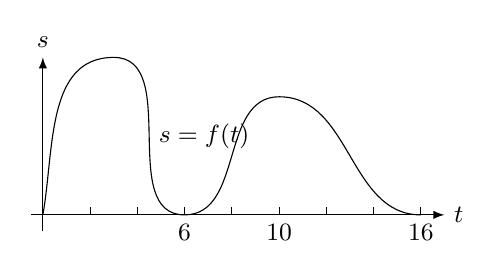
\begin{tikzpicture}[x=0.3cm,font=\small]
\draw[-latex](-0.5,0)--(17,0)node[right]{$t$};
\draw[-latex](0,-0.2)--(0,2)node[above]{$s$};
\foreach \x in {2,4,6,8,10,12,14,16}{\draw(\x,0)--++(0,0.1);}
\foreach \x in {6,10,16}{\draw(\x,0)node[below]{$\x$};}
\draw(0,0) to [out=80,in=180](3,2) to [out=0,in=180] node[pos=0.5,right]{$s=f(t)$}(6,0) to [out=0,in=180](10,1.5)to [out=0,in=180](16,0);
\end{tikzpicture}
\caption{ترسیم برائے سوال \حوالہ{سوال_استعمال_فاصلہ_وقت}}
\label{شکل_سوال_استعمال_فاصلہ_وقت}
\end{minipage}\hfill
\begin{minipage}{0.45\textwidth}
\centering
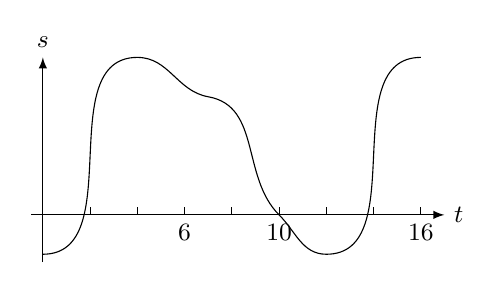
\begin{tikzpicture}[x=0.3cm,font=\small]
\draw[-latex](-0.5,0)--(17,0)node[right]{$t$};
\draw[-latex](0,-0.6)--(0,2)node[above]{$s$};
\foreach \x in {2,4,6,8,10,12,14,16}{\draw(\x,0)--++(0,0.1);}
\foreach \x in {6,10,16}{\draw(\x,0)node[below]{$\x$};}
\draw(0,-0.5) to [out=0,in=180](4,2) to [out=0,in=170](7,1.5) to [out=-10,in=135] (10,0) to [out=-45,in=180](12,-0.5) to [out=0,in=180](16,2);
\end{tikzpicture}
\caption{ترسیم برائے سوال \حوالہ{سوال_استعمال_فاصلہ_وقت_دوم}}
\label{شکل_سوال_استعمال_فاصلہ_وقت_دوم}
\end{minipage}
\end{figure}
\انتہا{سوال}
%==============
\ابتدا{سوال}\شناخت{سوال_استعمال_فاصلہ_وقت}\ترچھا{سمتی رفتار اور اسراع}\\
محددی لکیر پر آگے پیچے حرکت کرتے ہوئے جسم کا مقام بالمقابل وقت  شکل \حوالہ{شکل_سوال_استعمال_فاصلہ_وقت} میں دکھایا گیا ہے۔ (ا) جسم مبدا سے کب دور اور  کب مبدا کی طرف حرکت کرتا ہے؟  (ب) کب سمتی رفتار صفر ہے؟ (ج) کب اسراع صفر ہے؟ (د)  کب اسراع مثبت اور کب منفی ہے؟ 
\انتہا{سوال}
%========================
\ابتدا{سوال}\شناخت{سوال_استعمال_فاصلہ_وقت_دوم}\ترچھا{سمتی رفتار اور اسراع}\\
محددی لکیر پر آگے پیچے حرکت کرتے ہوئے جسم کا مقام بالمقابل وقت  شکل \حوالہ{شکل_سوال_استعمال_فاصلہ_وقت_دوم} میں دکھایا گیا ہے۔ (ا) جسم مبدا سے کب دور اور  کب مبدا کی طرف حرکت کرتا ہے؟  (ب) کب سمتی رفتار صفر ہے؟ (ج) کب اسراع صفر ہے؟ (د)  کب اسراع مثبت اور کب منفی ہے؟ 
\انتہا{سوال}
%========================
\ابتدا{سوال}\شناخت{سوال_استعمال_حاشیہ_الف}\ترچھا{حاشیہ لاگت}\\
\عددی{x} اشیاء پیدا کرنے پر لاگت \عددی{c=f(x)} کو شکل \حوالہ{شکل_سوال_استعمال_حاشیہ_الف} میں ترسیم کیا گیا ہے۔ کتنی پیداوار پر حاشیہ لاگت گھٹنے سے بڑھنا شروع ہوتی ہے؟\\
جواب:\quad
تقریباً \عددی{60}  پیدا وار پر۔
\انتہا{سوال}
%=========================
\ابتدا{سوال}\شناخت{سوال_استعمال_حاشیہ_ب}
ماہانہ آمدنی \عددی{y=r(t)} بالمقابل مہینہ کو شکل \حوالہ{شکل_سوال_استعمال_حاشیہ_ب} میں ترسیم کیا گیا ہے۔ کس دوران حاشیہ آمدنی بڑھ رہی ہے اور کب گھٹ رہی ہے؟
\انتہا{سوال}
%=====================
\begin{figure}
\centering
\begin{minipage}{0.45\textwidth}
\centering
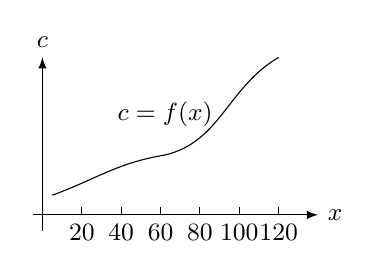
\begin{tikzpicture}[font=\small,x=0.5cm]
\draw[-latex](-0.25,0)--(7,0)node[right]{$x$};
\draw[-latex](0,-0.2)--(0,2)node[above]{$c$};
\foreach \x/\s in {1/20,2/40,3/60,4/80,5/100,6/120}{\draw(\x,0)node[below]{\s}--++(0,0.1);}
\draw(0.25,0.25) to [out=20,in=-170](3,0.75) to [out=10,in=-150]node[left]{$c=f(x)$}(6,2);
\end{tikzpicture}
\caption{لاگت بالمقابل پیداوار (سوال \حوالہ{سوال_استعمال_حاشیہ_الف})}
\label{شکل_سوال_استعمال_حاشیہ_الف}
\end{minipage}\hfill
\begin{minipage}{0.45\textwidth}
\centering
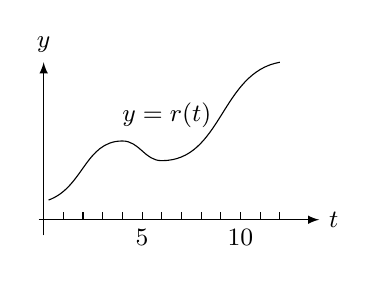
\begin{tikzpicture}[font=\small,x=0.25cm]
\draw[-latex](-0.25,0)--(14,0)node[right]{$t$};
\draw[-latex](0,-0.2)--(0,2)node[above]{$y$};
\foreach \x in {1,2,3,4,5,6,7,8,9,10,11,12}{\draw(\x,0)--++(0,0.1);}
\foreach \x in {5,10}{\draw(\x,0)node[below]{$\x$};}
\draw(0.25,0.25) to [out=20,in=180](4,1) to [out=0,in=180](6,0.75) to [out=0,in=-170]node[pos=0.5,left]{$y=r(t)$}(12,2);
\end{tikzpicture}
\caption{آمدن بالمقابل سال (سوال \حوالہ{سوال_استعمال_حاشیہ_ب})}
\label{شکل_سوال_استعمال_حاشیہ_ب}
\end{minipage}
\end{figure}

\ابتدا{سوال}
تفاعل \عددی{y=f(x)} کا تفرق درج ذیل ہے۔کہاں مقامی کم سے کم، مقامی زیادہ سے زیادہ یا  نقطہ تصریف پایا جاتا ہے؟(اشارہ: \عددی{y'} کی علامت کا نقش) 
\begin{align*}
y'=(x-1)^2(x-2)
\end{align*}
\انتہا{سوال}
%=======================
\ابتدا{سوال}
تفاعل \عددی{y=f(x)} کا تفرق درج ذیل ہے۔کہاں مقامی کم سے کم، مقامی زیادہ سے زیادہ یا  نقطہ تصریف پایا جاتا ہے؟(اشارہ: \عددی{y'} کی علامت کا نقش) 
\begin{align*}
y'=(x-1)^2(x-2)(x-4)
\end{align*}
\انتہا{سوال}
%=======================
\ابتدا{سوال}
\عددی{x>0} کے لئے ایسا تفاعل \عددی{y=f(x)} ترسیم کرین جس کا \عددی{f(1)=0} اور \عددی{f'(x)=\tfrac{1}{x}} ہے۔ کیا تفاعل کی مقعر کے بارے میں کچھ کہنا ممکن ہو گا؟ اپنے جواب کی وجہ پیش کریں۔
\انتہا{سوال}
%======================
\ابتدا{سوال}
تفاعل \عددی{y=f(x)} کا دودرجی تفرق استمراری اور غیر صفر ہے۔ کیا اس کی ترسیم کے بارے میں کطھ کہنا ممکن ہو گا؟ اپنے جواب کی وجہ پیش کریں۔
\انتہا{سوال}
%======================
\ابتدا{سوال}
مستقل \عددی{b}، \عددی{c} اور \عددی{d} کی صورت میں \عددی{b} کی کس قیمت کے لئے منحنی \عددی{y=x^3+bx^2+cx+d} کا نقطہ تصریف \عددی{x=1} پر پایا جائے گا؟ اپنے جواب کی وجہ پیش کریں۔
\انتہا{سوال}
%==========================
\ابتدا{سوال}\ترچھا{افقی ممام۔ درست یا غلط؟ سمجھائیں}
\begin{enumerate}
\item
ہر ایسے کثیر رکنی جس میں سب سے زیادہ طاقت جفت ہو  کا کم سے کم ایک افقی مماس پایا جاتا ہے۔
\item
ہر ایسے کثیر رکنی جس میں سب سے زیادہ طاقت طاق ہو  کا کم سے کم ایک افقی مماس پایا جاتا ہے۔
\end{enumerate}
\انتہا{سوال}
%=======================
\ابتدا{سوال}\ترچھا{قطع مکافی}
\begin{enumerate}
\item
قطع مکافی \عددی{y=ax^2+bx+c,\, a\ne 0} کا کنگرہ تلاش کریں۔
\item
قطع مکافی کب اوپر مقعر اور کب  نیچے مقعر ہے؟ اپنے جواب کی وجہ پیش کریں۔
\end{enumerate}
\انتہا{سوال}
%==========================
\ابتدا{سوال}
کیا یہ درست ہے کہ دو مرتبہ قابل تفرق تفاعل \عددی{y=f(x)} کی مقعر ہر ایسے نقطہ پر تبدیل ہوتی ہے جہاں \عددی{f''(x)=0} ہو؟ اپنے جواب کہ وجہ پیش کریں۔
\انتہا{سوال}
%==========================
\ابتدا{سوال}\ترچھا{دو درجی منحنی۔}\quad
آپ دو درجی منحنی \عددی{y=ax^2+bx+c,\, a\ne 0} کے نقطہ تصریف کے بارے میں کیا کہہ سکتے ہیں؟ اپنے جواب کی وجہ پیش کریں۔
\انتہا{سوال}
%================================
\ابتدا{سوال}\ترچھا{کعبی منحنی۔}\quad
آپ کعبی منحنی \عددی{y=ax^3+bx^2+cx+d,\, a\ne 0} کے نقطہ تصریف کے بارے میں کیا کہہ سکتے ہیں؟ اپنے جواب کی وجہ پیش کریں۔
\انتہا{سوال}
%================================
\موٹا{کمپیوٹر کا استعمال}\\
سوال \حوالہ{سوال_استعمال_کمپیوٹر_نقطہ_تصریف_الف} تا سوال \حوالہ{سوال_استعمال_کمپیوٹر_نقطہ_تصریف_ب} میں تفاعل کی ترسیم پر نقطہ تصریف (اگر موجود ہو)، مقامی کم سے کم اور مقامی زیاسدہ سے زیادہ نقطے  تلاش کریں۔ تفاعل کو ترسیم کرتے ہوئے ان نقطوں کی نشاندہی کریں۔ ساتھ ہی تفاعل کا یک درجی تفرق اور دو درجی تفرق بھی ترسیم کریں۔ جہاں یہ ترسیمات \عددی{x} محدد کو قطع کرتی ہیں، ان کا تفاعل کے ساتھ کیا تعلق ہے؟ اس کے علاوہ تفرق کے تفاعل کے ترسیم کے ساتھ کیا تعلقات ہیں؟ 

\ابتدا{سوال}\شناخت{سوال_استعمال_کمپیوٹر_نقطہ_تصریف_الف}
$y=x65-5x64-240$
\انتہا{سوال}
%==========================
\ابتدا{سوال}
$y=x^3-12x^2$
\انتہا{سوال}
%========================
\ابتدا{سوال}
$y=\tfrac{4}{5}x^5+16x^2-25$
\انتہا{سوال}
%========================
\ابتدا{سوال}\شناخت{سوال_استعمال_کمپیوٹر_نقطہ_تصریف_ب}
$y=\tfrac{x^4}{4}-\tfrac{x^3}{3}-4x^2+12x+20$
\انتہا{سوال}
%========================
\ابتدا{سوال}
تفاعل \عددی{f(x)=2x^4-4x^2+1} اور اس کے پہلے دو تفرق ایک ساتھ ترسیم کریں۔ \عددی{f'} اور \عددی{f''} کی قیمتوں اور علامتوں کے لحاظ سے \عددی{f} کے رویہ پر بحث کریں۔
\انتہا{سوال}
%=====================
\ابتدا{سوال}
تفاعل \عددی{f(x)=x\cos x} اور اس کے پہلے دو تفرق کو \عددی{0\le x\le 2\pi} کے لئے ایک ساتھ ترسیم کریں۔ \عددی{f''} کی قیمتوں اور علامتوں کے لحاظ سے \عددی{f} کے رویہ پر بحث کریں۔
\انتہا{سوال}
%=====================
\ابتدا{سوال}
\begin{enumerate}
\item
\عددی{k=0} اور  اس کی قریبی مثبت اور منفی قیمتوں کے لئے \عددی{f(x)=x^3+kx} کو ایک ساتھ ترسیم کریں۔\عددی{k} کی قیمت کا ترسیم کی صورت پر کیا اثر پایا جاتا ہے؟
\item
\عددی{f''(x)} تلاش کریں۔آپ دیکھیں گے کہ \عددی{f''(x)} دو درجی مساوات ہے۔ \عددی{f''(x)} کا ممیز تلاش کریں (\عددی{ax^2+bx+c} کا ممیز \عددی{b^2-4ac} ہے)۔ \عددی{k} کی کن قیمتوں کے لئے ممیز مثبت ہے؟ صفر ہے؟ منفی ہے؟ \عددی{k} کی کن قیمتوں کے لئے \عددی{f'(x)} کے  صفروں کی تعداد دو ہے؟ ایک ہے؟  صفر ہے؟ اب بتائیں کہ \عددی{k} کی قیمت کا \عددی{f(x)} کی ترسیم کی صورت کے ساتھ کیا تعلق ہے۔
\item
\عددی{k} کی دیگر قیمتوں کے ساتھ تجربہ کر کے دیکھیں۔ \عددی{k\to \infty} اور \عددی{k\to -\infty} کرنے سے کیا ہوتا ہے؟
\end{enumerate}
\انتہا{سوال}
%=======================
\ابتدا{سوال}
\begin{enumerate}[a.]
\item
\عددی{k=-4} اور اس کے قریبی قیمتوں کے لئے  ایک ساتھ \عددی{-1\le x\le 4} پر \عددی{f(x)=x^4+kx^3+6x^2} ترسیم کریں۔ \عددی{k} کی قیمت ترسیم کی صورت پر کس طرح اثر انداز ہوتی ہے؟
\item
\عددی{f''(x)} تلاش کریں۔آپ دیکھیں گے کہ \عددی{f''(x)} دو درجی مساوات ہے۔ \عددی{f''(x)} کا ممیز تلاش کریں (\عددی{ax^2+bx+c} کا ممیز \عددی{b^2-4ac} ہے)۔ \عددی{k} کی کن قیمتوں کے لئے ممیز مثبت ہے؟ صفر ہے؟ منفی ہے؟ \عددی{k} کی کن قیمتوں کے لئے \عددی{f'(x)} کے  صفروں کی تعداد دو ہے؟ ایک ہے؟  صفر ہے؟ اب بتائیں کہ \عددی{k} کی قیمت کا \عددی{f(x)} کی ترسیم کی صورت کے ساتھ کیا تعلق ہے۔
\end{enumerate}
\انتہا{سوال}
%=================
\ابتدا{سوال}
\begin{enumerate}[a.]
\item
\عددی{-3\le x\le 3} کے لئے \عددی{y=x^{2/3}(x^2-2)} ترسیم کریں۔اس کے بعد احصاء کی استعمال سے مقعر، اٹھان اور نیچے گرنے کی تصدیق کریں۔
\item
کیا \عددی{x=0} پر منحنی کا کنگرہ پایا جاتا ہے یا صرف ایک کونا جس کے بائیں ہاتھ اور دائیں ہاتھ تفرق مختلف ہیں؟
\end{enumerate}
\انتہا{سوال}
%=====================
\ابتدا{سوال}
\begin{enumerate}[a.]
\item
\عددی{-0.5\le x\le  1.5} پر \عددی{y=9x^{2/3}(x-1)} ترسیم کریں۔ اس کے بعد احصاء کی مدد سے مقعر، مقامی کم سے کم اور مقامی زیادہ سے زیادہ نقطوں کی تصدیق کریں۔ مبدا کے بائیں جانب کون سی مقعر ہے؟
\item
کیا \عددی{x=0} پر ترسیم کا کنگرہ پایا  جاتا ہے یا صرف ایک کونا جس کے بائیں ہاتھ اور دائیں ہاتھ تفرق مختلف ہیں؟
\end{enumerate}
\انتہا{سوال}
%========================
\ابتدا{سوال}
کیا \عددی{x=-3} کے قریب \عددی{y=x^2+3\sin 2x} کا افقی مماس پایا جاتا ہے؟ اپنے جواب کی وجہ پیش کریں۔
\انتہا{سوال}
%===========================

\حصہ{حد؟؟؟؟}
